\documentclass{article}
\PassOptionsToPackage{numbers,sort&compress}{natbib}
\usepackage[preprint,main]{neurips_2026}
\usepackage[T1]{fontenc}
\usepackage[utf8]{inputenc}
\usepackage{amsmath,amssymb,mathtools,booktabs,multirow}
\usepackage{graphicx,subcaption,algorithm,algpseudocode}
\usepackage{tikz}
\usetikzlibrary{arrows.meta,positioning,fit,backgrounds,calc}
\usepackage{xcolor,microtype,url}
\usepackage[colorlinks=true,linkcolor=teal!65!black,citecolor=teal!65!black,urlcolor=teal!65!black]{hyperref}
\definecolor{agentblue}{HTML}{147D92}
\definecolor{agentorange}{HTML}{C85B39}
\definecolor{ink}{HTML}{183044}
\newcommand{\D}{\mathcal{D}}
\newcommand{\U}{\mathcal{U}}
\newcommand{\low}{\mathrm{low}}
\newcommand{\rand}{\mathrm{rand}}
\newcommand{\pp}{\,\mathrm{pp}}
\newcommand{\ind}{\mathbb{1}}
\newcommand{\smallpara}[1]{\paragraph{#1}}
\graphicspath{{figures/}}
\newcommand{\SelectionRows}{%
Task matched & API & 27.930 & 10.156 & -17.773 & 1/0/15 \\%
Task matched & GENERIC & 12.695 & 4.883 & -7.812 & 5/0/11 \\%
Task + action & API & 31.706 & 26.888 & -4.818 & 8/1/15 \\%
Task + action & GENERIC & 6.771 & 3.776 & -2.995 & 3/6/15 \\%
}

\newcommand{\InitializationRows}{%
101 & -5.859 & -1.562 \\%
202 & -10.156 & -3.125 \\%
303 & -2.344 & -2.734 \\%
404 & +0.000 & -4.297 \\%
505 & -1.562 & -1.953 \\%
606 & -8.984 & -4.297 \\%
}

\title{When Low-Loss Demonstrations Hurt:\\Controlled Experience Selection for Language Agents}
\author{Anonymous Authors}
\date{}
\begin{document}
\raggedbottom
\maketitle
\begin{abstract}
An agent's successful experience need not be useful training data for its underlying model. We study this distinction in supervised fine-tuning of a 4B language agent in ALFWorld, separating collection conditions, experience selection, and post-training execution. A sequence of controlled comparisons first holds training dose fixed, then matches task exposure and distinct-content budgets, and finally matches task-by-action composition. At equal presentation and update budgets, a complete-pass schedule improves task success over subset replay by 5.18 and 1.27 percentage points in two historical source pools. Under task matching, selecting actions with low base-student negative log-likelihood instead of random selection reduces mean success by 17.77 and 7.81 points across four initialization/dropout seeds and four sampling recipes. After task-by-action matching, negative average differences remain: 4.82 and 2.99 points across six initialization seeds. We report every paired cell, conditional retrains, and independent scoring checks. Uniform rescoring changes 4--11 of 256 selected records per recipe; its downstream replication is ongoing and excluded from the results. These findings provide a controlled failure case for an action-level predictability proxy, with explicit limits from one backbone, finite source pools, and reused development tasks.
\end{abstract}

\section{Introduction}
\label{sec:intro}
Language agents solve tasks through repeated interaction with an environment. Their performance depends on both model parameters and the surrounding harness: demonstrations, planning instructions, external guidance, and execution rules. ReAct exemplifies how a prompting and interaction protocol can improve behavior without updating parameters~\citep{yao2023react}. When the resulting experience is used for fine-tuning, however, the relevant question changes: \emph{which experience improves the student after collection-specific assistance is withdrawn?}

Three quantities must be distinguished. Collection success measures the collecting system. A selection score measures a property of candidate experience. Post-training task success measures the updated student under a specified executor. A successful episode can contain redundant actions, and an action that the base student already predicts well can provide little useful supervision. Conversely, an initially surprising action may expose a behavior the student needs to acquire. These possibilities motivate direct intervention on the training experience rather than inferring its value from collection success or likelihood alone.

We study a deliberately narrow comparison: random selection versus selection of low base-student action negative log-likelihood (NLL) examples from the same historical pool. The selection unit is an action demonstration with its genuine preceding history, rather than an independently generated complete trajectory. This distinction matters when relating the comparison to trajectory-level distillation~\citep{tang2026smartad} or methods that estimate reference-relative loss and gradient influence~\citep{lin2024rho,xia2024less}.

Our experimental protocol progressively constrains experience composition. We first compare complete-pass exposure with subset replay at a fixed optimization budget. We then compare selection policies while matching task identity at every presentation and the distinct-content budget. Finally, we match task-by-action positions and within-stratum distinct-content quotas. Across the two fixed source pools, low-NLL selection is worse on average under both selection controls. Matching action composition reduces the observed gaps, but also changes the support and strength of the intervention; this reduction is not an identified mediation estimate.

\begin{figure}[t]
  \centering
  \resizebox{\linewidth}{!}{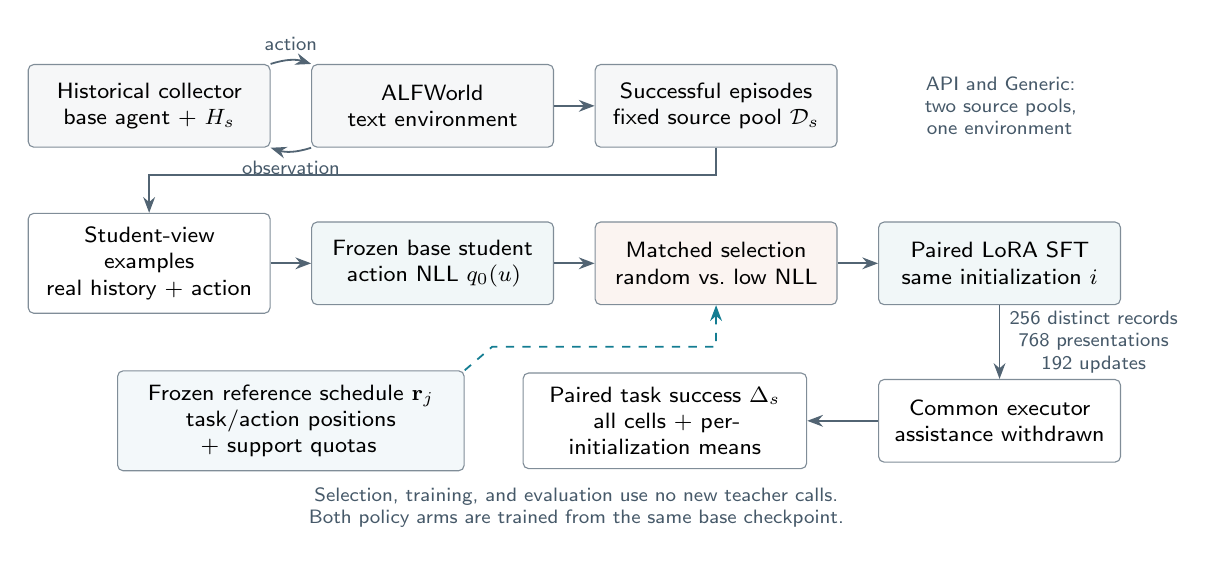
\begin{tikzpicture}[
  font=\sffamily\footnotesize,
  block/.style={draw=ink!55,rounded corners=2pt,align=center,text width=2.72cm,minimum height=1.05cm,inner sep=5pt,fill=white},
  flow/.style={-{Stealth[length=2mm]},line width=.65pt,draw=ink!75},
  control/.style={flow,dashed,draw=agentblue},
  note/.style={align=center,font=\sffamily\scriptsize,text=ink!80}]
\node[block,fill=ink!4] (harness) at (0,0) {Historical collector\\base agent + $H_s$};
\node[block,fill=ink!4] (env) at (3.6,0) {ALFWorld\\text environment};
\node[block,fill=ink!4] (pool) at (7.2,0) {Successful episodes\\fixed source pool $\D_s$};
\node[note,text width=2.7cm] at (10.8,0) {API and Generic:\\two source pools,\\one environment};
\draw[flow] (harness.north east) to[bend left=18] node[above,note]{action} (env.north west);
\draw[flow] (env.south west) to[bend left=18] node[below,note]{observation} (harness.south east);
\draw[flow] (env) -- (pool);
\node[block] (view) at (0,-2.0) {Student-view examples\\real history + action};
\node[block,fill=agentblue!6] (score) at (3.6,-2.0) {Frozen base student\\action NLL $q_0(u)$};
\node[block,fill=agentorange!7] (select) at (7.2,-2.0) {Matched selection\\random vs.\ low NLL};
\node[block,fill=agentblue!6] (train) at (10.8,-2.0) {Paired LoRA SFT\\same initialization $i$};
\draw[flow] (pool.south) -- ++(0,-.35) -| (view.north);
\draw[flow] (view) -- (score);
\draw[flow] (score) -- (select);
\draw[flow] (select) -- (train);
\node[block,text width=4.05cm,fill=agentblue!5] (quotas) at (1.8,-4.0) {Frozen reference schedule $\mathbf r_j$\\task/action positions + support quotas};
\node[block,text width=3.25cm] (result) at (6.55,-4.0) {Paired task success $\Delta_s$\\all cells + per-initialization means};
\node[block] (eval) at (10.8,-4.0) {Common executor\\assistance withdrawn};
\draw[control] (quotas.north east) -- ++(.35,.30) -| (select.south);
\draw[flow] (train) -- node[right,note]{256 distinct records\\768 presentations\\192 updates} (eval);
\draw[flow] (eval) -- (result);
\node[note,text width=12.8cm] at (5.4,-5.1) {Selection, training, and evaluation use no new teacher calls. Both policy arms are trained from the same base checkpoint.};
\end{tikzpicture}
}
  \caption{\textbf{Study architecture.} Historical collection supplies fixed experience pools. We rebuild genuine student-view examples, score them with the frozen base model, and intervene on selection under shared reference constraints. Both policy arms receive the same optimization budget and are evaluated through a common executor after collection-specific assistance is removed. Source labels are collection conditions, not randomized harness treatments.}
  \label{fig:architecture}
\end{figure}

We make three contributions. First, we formalize a reproducible selection comparison that separates training dose, task exposure, distinct content, and action composition. Second, we report completed comparisons across crossed initialization and sampling seeds, including positive paired cells and conditional retrains. Third, we audit numerical scoring consistency independently of downstream training, showing why selection overlap alone cannot establish performance robustness. The evidence supports a concrete failure case for this action-level proxy. It does not establish a general optimal selector, harness superiority, or a transferable learning mechanism.


\section{Related Work}
\label{sec:related}
\smallpara{Interactive agents and learning from assistance.}
ALFWorld aligns textual household interaction with embodied tasks~\citep{shridhar2021alfworld}; our experiments use its text interface. WebShop evaluates grounded shopping decisions in a simulated website~\citep{yao2022webshop}. ReAct combines reasoning and actions through public demonstrations~\citep{yao2023react}. More recent work explicitly studies skill-guided training and skill-free deployment: SkillScaffold estimates policy-relative skill utility and selectively injects skills during agentic RL~\citep{zhong2026skillscaffold}. Our controlled SFT comparison holds the historical pool fixed and changes which action examples receive a finite training budget. It neither reproduces SkillScaffold nor tests an RL update rule.

\smallpara{Predictability and data selection.}
SmartAD selects a correct teacher trajectory with low student NLL and additionally changes segment-level supervision weights~\citep{tang2026smartad}. Our action-level selection omits those trajectory and weighting components. Rho-1 uses reference-based selective token training~\citep{lin2024rho}, while LESS uses optimizer-aware gradient features and target demonstrations~\citep{xia2024less}. These methods differ in selection unit, available information, and cost; raw action NLL is not a substitute for implementing them. Our results delimit one proxy under controlled interactive-agent fine-tuning, rather than refute student-aligned selection in general.

\smallpara{Selection, updates, and evaluation.}
EvoHeir separates task admission, parameter inheritance, and experience inheritance, emphasizing that a promising selected task need not yield a useful update~\citep{yang2026evoheir}. Our comparison isolates selection from a fixed experience pool rather than choosing which updated model to inherit. More broadly, few-run RL evaluation can be sensitive to the analysis procedure~\citep{agarwal2021precipice}. We therefore expose crossed seed roles and every paired cell, and restrict the current claims to descriptive results on fixed development tasks.

\section{A Controlled Experience-Selection Protocol}
\label{sec:method}
\subsection{Examples, predictability, and training schedules}
A fixed source pool $\D_s$ contains eligible action demonstrations $z=(x,h,a)$: task $x$, actual public interaction history $h$, and the next canonical action $a$. Here $a$ includes the supervised JSON serialization and its chat-template terminator; $c(a)$ parses the command's action family. Let $u(z)$ identify the complete student-view messages by exact content. Deduplication identifies literal message equality, not semantic equivalence. Every retained example preserves its real history; selecting examples does not synthesize a new interaction trajectory.

For the frozen base student $p_{\theta_0}$, action predictability is measured by token-average target NLL,
\begin{equation}
 \ell_0(z)=-\frac{1}{|a|}\sum_{v=1}^{|a|}
 \log p_{\theta_0}(a_v\mid h,a_{<v}).
 \label{eq:nll}
\end{equation}
The original cache can assign different numerical values to identical content in different batching layouts. The completed selection experiments use the recorded mean over copies of each content identity,
\begin{equation}
 q_0(u)=\frac{1}{|\{z\in\D_s:u(z)=u\}|}
 \sum_{z\in\D_s:u(z)=u}\ell_0^{\mathrm{cache}}(z).
 \label{eq:cache}
\end{equation}
We retain that definition for the historical experiments; an independent uniform-scoring check is reported separately in Section~\ref{sec:scoring}.

A sampling recipe $j$ defines a frozen reference schedule $\mathbf r_j=(r_1,\ldots,r_B)$ with $B=768$ presentations. For a stratum function $g$, define the number of presentations and distinct content identities assigned to stratum $g$:
\begin{equation}
 n_g=\sum_{k=1}^{B}\ind\{g(z_{r_k})=g\},\qquad
 K_g=\left|\{u(z_{r_k}):g(z_{r_k})=g\}\right|.
 \label{eq:quotas}
\end{equation}
The two policies select $K_g$ identities from the eligible distinct support $\U_g$. Random selection samples uniformly without replacement; low-NLL selection solves
\begin{equation}
 A_g^{\low}\in\underset{A\subseteq\U_g,\,|A|=K_g}{\arg\min}
 \sum_{u\in A}q_0(u).
 \label{eq:selection}
\end{equation}
Ties are resolved by the representative corpus index. Within each stratum, a fixed recipe-specific shuffle cycles through the selected identities, visiting every identity before repeating it. These stratum sequences are interleaved in reference order. For the resulting policy schedule $\boldsymbol\sigma^{p}_{s,j}$,
\begin{align}
 g(z_{\sigma_k^p})&=g(z_{r_k})\quad &&\text{for every presentation }k,\label{eq:positions}\\
 \left|\{u(z_{\sigma_k^p}):g(z_{\sigma_k^p})=g\}\right|&=K_g\quad &&\text{for every stratum }g.\label{eq:support}
\end{align}
The selected content may differ while these constraints hold exactly.

\subsection{Progressively stronger controls}
\begin{figure}[t]
\centering
\resizebox{\linewidth}{!}{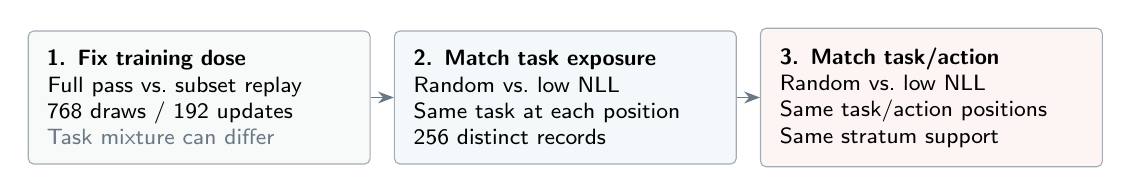
\begin{tikzpicture}[font=\sffamily\footnotesize,
 card/.style={draw=ink!40,rounded corners=2pt,align=left,text width=3.85cm,minimum height=1.65cm,inner sep=7pt},
 flow/.style={-{Stealth[length=2mm]},draw=ink!65,line width=.65pt}]
\node[card,fill=ink!3] (s2) at (0,0) {\textbf{1. Fix training dose}\\Full pass vs.\ subset replay\\768 draws / 192 updates\\\textcolor{ink!65}{Task mixture can differ}};
\node[card,fill=agentblue!5] (s3) at (4.65,0) {\textbf{2. Match task exposure}\\Random vs.\ low NLL\\Same task at each position\\256 distinct records};
\node[card,fill=agentorange!6] (s4) at (9.3,0) {\textbf{3. Match task/action}\\Random vs.\ low NLL\\Same task/action positions\\Same stratum support};
\draw[flow] (s2) -- (s3);
\draw[flow] (s3) -- (s4);
\end{tikzpicture}
}
\caption{\textbf{Progressive controls, not interchangeable treatments.} Each comparison answers a different conditional question. The final constraint also restricts eligible content support and weakens the low-NLL selection contrast; changes in effect size across stages cannot be read as a mediation fraction.}
\label{fig:controls}
\end{figure}
\smallpara{Training dose: complete pass versus subset replay.}
Both arms receive 768 presentations and 192 updates. Complete-pass scheduling traverses the eligible corpus before repeating rows; the replay arm reuses a 256-row subset. Membership, multiplicity, order, and task mixture can change together. This first comparison evaluates the scheduling intervention as a whole.

\smallpara{Task-matched selection.}
We set $g(z)=x$. The policies share task identity at every presentation, task counts, and 256 distinct task/content records. They can still differ in action composition. We cross four initialization/dropout seeds with four sampling recipes within each source.

\smallpara{Task-by-action-matched selection.}
We set $g(z)=(x,c(a))$ and inherit the task/action quotas from the task-matched random reference. The policies now share every task/action position and within-stratum support count. Action families absent from the reference remain absent. The support restriction retains approximately 66.15\% and 40.44\% of the preceding NLL-selection contrast in the API and Generic pools. It changes the intervention as well as the control. We cross six initialization/dropout seeds with the same four sampling recipes.

\begin{algorithm}[t]
\caption{Matched content selection and paired evaluation}
\label{alg:protocol}
\begin{algorithmic}[1]
\Require Fixed pool $\D_s$, base student $\theta_0$, reference $\mathbf r_j$, strata $g$
\State Compute content identities, scores $q_0(u)$, and quotas $(n_g,K_g)$
\For{$p\in\{\rand,\low\}$}
  \State Select $A_g^p$ independently within each reference stratum
  \State Cycle shuffled identities within each stratum; interleave in reference order
  \State Verify Eqs.~\eqref{eq:positions}--\eqref{eq:support}, total support, and schedule hashes
  \For{initialization/dropout seed $i$}
    \State Train a fresh LoRA adapter on $\boldsymbol\sigma^p_{s,j}$ for 192 updates
    \State Audit weights and evaluate through the common executor without collection guidance
  \EndFor
\EndFor
\State Report paired differences, all initialization means, and all wins/ties/losses
\end{algorithmic}
\end{algorithm}

\subsection{Training and estimands}
We fine-tune low-rank adapters~\citep{hu2022lora} while freezing the backbone. The supervised objective averages the token-normalized target loss over scheduled examples,
\begin{equation}
 \mathcal L(\phi;\boldsymbol\sigma)
 =\frac1B\sum_{k=1}^{B}\ell_{\theta_0+\Delta(\phi)}(z_{\sigma_k}).
 \label{eq:sft}
\end{equation}
The implementation uses microbatches of one example and gradient accumulation to a global batch of four. Both policies use the same initialization/dropout seed $i$, optimizer configuration, and update budget. Equal presentations do not imply identical input/target token totals or exact FLOPs.

Let $Y_{s,p,i,j,f,t}$ denote success for source $s$, policy $p$, initialization $i$, recipe $j$, family $f$, and task $t$. Each model's outcome and the primary contrast are
\begin{align}
 R_{s,p,i,j}&=\frac12\sum_{f\in\{\mathrm{cool},\mathrm{heat}\}}
                  \frac1{32}\sum_{t=1}^{32}Y_{s,p,i,j,f,t},\label{eq:success}\\
 \Delta_s&=\frac1{IJ}\sum_{i=1}^{I}\sum_{j=1}^{J}
                (R_{s,\low,i,j}-R_{s,\rand,i,j}).\label{eq:effect}
\end{align}
Initialization seeds and sampling recipes are crossed factors. We also report $\Delta_{s,i}=J^{-1}\sum_j(R_{s,\low,i,j}-R_{s,\rand,i,j})$. The 24 task/action-matched cells are not 24 independent initialization seeds. Conditional repeats are excluded from these primary means.

\section{Experiments}
\label{sec:experiments}
\subsection{Setting and evaluation protocol}
We use Qwen3-4B-Instruct-2507 from the Qwen3 family~\citep{yang2025qwen3}, with a pinned revision recorded in Appendix~\ref{app:inventory}. The two historical experience pools, API and Generic, contain 721/732 eligible action rows from 35/29 collection tasks and 418/508 exact distinct message records. These labels describe existing collection conditions; the main contrasts are \emph{within} a source. The pools are not independent environments or randomized harness treatments. No new teacher calls are made in the controlled selection studies.

Training uses BF16 LoRA with rank 16, alpha 32, dropout 0.05, attention projections $q,k,v,o$, learning rate $10^{-4}$, zero weight decay, 0.05 warmup ratio, and maximum sequence length 2,048. Both policies receive 192 updates and 768 presentations. The task-matched comparison has 64 primary models, four conditional retrains, and two fresh full-pass reference checks. The task/action-matched comparison has 96 primary models and four conditional retrains. A paired policy cell shares a physical GPU; every source/policy group in the latter study has 12 primary models on each of two RTX 5090s.

Evaluation uses 32 cooling and 32 heating development tasks, environment seed 11, temperature zero, batch size eight, and a common JSON executor. Collection-specific assistance is removed; fixed public execution instructions and examples remain. The audited checkpoint combines the trained A adapter with an untrained zero-effect B adapter at step zero. These are repeatedly inspected development tasks from the official training pool. Official seen/unseen tests remain sealed. We report descriptive paired outcomes rather than uncalibrated confidence intervals or significance claims.

\begin{table}[t]
\centering
\caption{\textbf{Completed selection comparisons.} Success rates are percentages; $\Delta$ is low NLL minus random in percentage points. W/T/L counts paired initialization--recipe cells, not independent initialization seeds. Conditional retrains are excluded.}
\label{tab:main}
\small
\begin{tabular}{llrrrr}
\toprule
Control & Source & Random & Low NLL & $\Delta$ (pp) & W/T/L\\
\midrule
\SelectionRows
\bottomrule
\end{tabular}
\end{table}

\subsection{Experience support at a fixed training dose}
\label{sec:dose}
The complete-pass versus subset-replay study completes 68 new models and 4,352 evaluation episodes. At 768 presentations and 192 updates, complete-pass exposure increases mean success by 5.176 points for API and 1.270 points for Generic. The source-contrast sampling standard deviations within the four initialization blocks change from 8.87/13.46/18.55/19.36 to 3.83/6.31/5.90/2.34 points. These values describe four recipes per block, not population variance intervals. Since the intervention can also change task mixtures and multiplicities, we next constrain task exposure directly.

\subsection{Low action NLL under matched task exposure}
\label{sec:task}
The task-matched study completes all 70 new models and 4,480 evaluation episodes. Its primary comparison uses four initialization seeds crossed with four recipes for each source and policy. Random and low-NLL schedules share task position, task counts, and 256 distinct task/content records. Low-NLL selection lowers mean success from 27.930\% to 10.156\% in API and from 12.695\% to 4.883\% in Generic (Table~\ref{tab:main}). Every initialization-level average is negative in both pools.

The means do not imply uniform harm. One of 16 API cells and five of 16 Generic cells favor low NLL. Figure~\ref{fig:outcomes} retains these cells rather than replacing the distribution by a single mean. Action composition remains free to vary, so this comparison cannot attribute the difference to content properties beyond action distribution.

\begin{figure}[t]
  \centering
  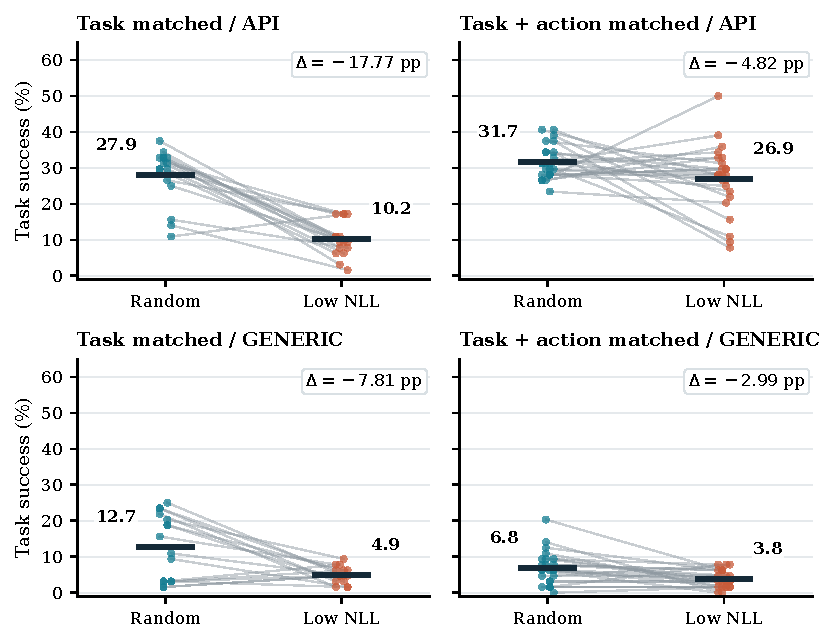
\includegraphics[width=\linewidth]{selection-outcomes.pdf}
  \caption{\textbf{Every primary paired cell.} Lines connect random and low-NLL outcomes for one initialization--recipe pair; black ticks show means. Top: API; bottom: Generic. Left: task matching (16 pairs per source). Right: task/action matching (24 pairs per source). All panels use the same vertical scale. No confidence interval is encoded. Lines sharing an initialization are not independent training seeds.}
  \label{fig:outcomes}
\end{figure}

\subsection{Residual differences after action-composition matching}
\label{sec:action}
The task/action-matched study completes 100 models and 6,400 evaluation episodes, using 14.663 cumulative GPU-hours against an 18-hour cap. The 96 primary models cover six initialization/dropout seeds and four recipes. Low NLL remains worse on average: 31.706\% versus 26.888\% for API, and 6.771\% versus 3.776\% for Generic. API has five negative initialization-level means and one zero; Generic has six negative means. Paired W/T/L counts are 8/1/15 and 3/6/15, respectively.

The smaller gaps relative to task matching are informative constraints on the original observation, but do not identify how much of it was caused by action composition. The reference quotas change available content support and weaken the selection contrast. Absolute performance also changes differently across pools. A post-hoc comparison restricted to the first two initialization blocks changes API random/low-NLL success from 28.125\%/10.938\% to 32.031\%/24.023\%; Generic changes from 11.133\%/5.469\% to 6.250\%/3.906\%. Gap reduction can accompany improvement or deterioration in absolute success. Appendix~\ref{app:seeds} reports all initialization-level differences.

\subsection{Training variability and scoring consistency}
\label{sec:scoring}
Four prespecified conditional retrains in the final study use initialization 101, recipe 101, and the original physical GPUs. All four produce different final weights. Success changes are 0.000 and $-4.688$ points for API random and low NLL, and $+1.562$ and $-1.562$ for Generic. These repeated cells are separate from primary means and do not estimate a population variance. An earlier post-hoc check reevaluates two stored checkpoints under their original configurations, adding 128 episodes; each reproduces its own recorded success and step count. This does not establish universal evaluation determinism.

An independent scoring diagnostic completes 1,194 forward passes, including uniform scoring of all 853 distinct message inputs, in 107.127 GPU seconds. Canonical repeats and original-layout replays reproduce their respective scores exactly. Four checks against direct supervised loss have absolute discrepancy at most $3.54\times10^{-6}$. Padding/precision stress tests nevertheless reveal numerical differences. The 32 stress inputs were selected deliberately and are not a representative error sample.

Uniform scores change 4--11 of 256 selected records across 16 original recipes, retaining 95.703\%--98.438\% of the content. High overlap is not a downstream performance guarantee. A separately frozen, 96-model paired retraining study using uniform scores is running; its interim outcomes are excluded from all main-paper tables and figures. Appendix~\ref{app:scoring} reports the completed instrument checks.

\subsection{Source comparison and second-environment calibration}
\label{sec:scope}
The earlier teacher-assisted versus ReAct self-collection study is a separate estimand. Collection succeeds in 69/144 and 110/144 attempts, respectively. On 58 common successful task/seed pairs, its API-minus-ReAct raw adaptation-AUC difference is $-3.56$ points, with seed values $-9.77$, $-3.42$, and $+2.49$. This result is retained; within-pool selection results do not overturn it. Common-success matching discards unmatched coverage, and a sufficiently consumed full-eligible-data comparison remains open.

A WebShop base-model calibration completes 64 train-only episodes on 32 shared goals under two public prompt ports. ReAct solves 5/32 and Act-only solves 6/32; their mean partial scores are 0.4125 and 0.4380. All 463 requests finish without transport errors, but include 34 invalid-format and 136 invalid-control model decisions. The pilot verifies an executable second environment and measures headroom. It has no SFT intervention and is neither cross-environment replication of the selection effect nor a published benchmark comparison. Full details appear in Appendix~\ref{app:webshop}.

\section{Discussion and Limitations}
\label{sec:discussion}
\smallpara{What the controlled result establishes.}
At a fixed optimization dose, experience support affects task success. Even after matching task identity and distinct-content counts, low base-student action NLL is not a reliable selector in the two studied pools. A negative average remains under task/action matching. The result is a property of this selection rule, candidate support, student, and executor, rather than a theorem that easier examples are always harmful. Predictability and usefulness are different measurement targets, and these experiments show one setting in which they fail to align.

\smallpara{What the controls leave open.}
Matching action families does not equalize finer action semantics, context difficulty, recovery structure, or relevance to evaluation tasks. Restricting support also changes the NLL contrast. We therefore do not identify a causal mediation fraction or claim that these remaining features explain the result. A mechanism claim needs a measurable predictor that generalizes across collection conditions, followed by an intervention that changes outcomes while the established controls are retained.

\smallpara{Generalization and statistical uncertainty.}
The current evidence uses one backbone, two finite pools, and reused development tasks. Six initialization seeds improve visibility of conditional variation but do not replace new task identities. Formal binary-outcome interval calibration remains incomplete; we present all paired cells and per-initialization means without significance or equivalence claims. The evaluation executor is consequential: in the separate source study, base-model heating success changes from 6.25\% under JSON execution to 84.38\% under the stronger common ReAct executor. Fresh tasks, a common stronger executor, stronger selection baselines, and a second-environment learning intervention are needed before a broader benchmark claim.

\smallpara{Selection units and available candidates.}
Our selection unit is an action example with real history. A provenance audit traces 117 successful historical trajectories, but only two API tasks and one Generic task have multiple distinct, fully retained eligible complete trajectories. The old pools therefore offer little meaningful complete-trajectory choice. A trajectory-level baseline requires a new candidate pool; it cannot be manufactured by renaming the current action-level treatment.

\section{Conclusion}
We introduce and execute a progressively constrained experience-selection protocol for language-agent fine-tuning. Low action NLL is worse than random selection on average in two historical pools, including after task/action matching. Independent scoring and training-repeat audits expose practical boundaries of that observation. The next question is whether the controlled failure persists with uniform-score retraining, new tasks, stronger selectors, and an independent learning environment.


\bibliographystyle{plainnat}
{\small\bibliography{references}}
\clearpage
\appendix
\section{Experimental Inventory and Implementation}
\label{app:inventory}
Table~\ref{tab:inventory} distinguishes new model training from historical reference reuse and separate checkpoint checks. The three completed selection studies train 238 new models and execute 15,232 new policy-evaluation episodes in total. The scoring diagnostic generates no actions and performs no optimizer updates. WebShop base calibration adds 64 train-only episodes. These counts are not pooled as independent learning observations.

\begin{table}[h]
\centering
\caption{Completed study inventory. Additional references and conditional repeats are excluded from primary selection means.}
\label{tab:inventory}
\small
\begin{tabular}{lrrl}
\toprule
Study & New models & New episodes & Primary design / additional checks\\
\midrule
Complete pass vs.\ replay & 68 & 4,352 & 64 primary + 4 repeats\\
Task matching & 70 & 4,480 & 64 primary + 4 repeats + 2 references\\
Task/action matching & 100 & 6,400 & 96 primary + 4 repeats\\
Stored-checkpoint reevaluation & 0 & 128 & 2 checkpoints, original configurations\\
Uniform scoring diagnostic & 0 & 0 & 1,194 forwards; 853 distinct inputs\\
WebShop base calibration & 0 & 64 & 32 shared goals, two public prompts\\
\bottomrule
\end{tabular}
\end{table}

\begin{table}[h]
\centering
\caption{Shared configuration for the controlled selection studies.}
\label{tab:config}
\small
\begin{tabular}{ll}
\toprule
Parameter & Value\\
\midrule
Backbone & Qwen3-4B-Instruct-2507, fixed revision\\
Revision & \texttt{cdbee75f17c01a7cc42f958dc650907174af0554}\\
Training precision / adaptation & BF16 / LoRA\\
LoRA rank / alpha / dropout & 16 / 32 / 0.05\\
Trainable projections & \texttt{q\_proj}, \texttt{k\_proj}, \texttt{v\_proj}, \texttt{o\_proj}\\
Learning rate / weight decay & $10^{-4}$ / 0\\
Warmup ratio / maximum sequence & 0.05 / 2,048 tokens\\
Microbatch / gradient accumulation & 1 example / 4 microbatches\\
Updates / sample presentations & 192 / 768\\
Distinct task/content budget (selection) & 256 per model\\
Evaluation families & 32 cooling + 32 heating tasks, equal weights\\
Environment seed / temperature / batch & 11 / 0 / 8\\
Collection-specific guidance & Removed during evaluation\\
Official final evaluation sets & Unopened\\
\bottomrule
\end{tabular}
\end{table}

\smallpara{Checkpoint composition.}
The inherited evaluation path serves a trained A adapter plus an untrained B adapter at optimizer step zero. The B adapter has zero effect on the base prediction at initialization, but it remains part of the serialized composition. Audits verify the base revision, A-weight identity, zero-B reference identity, and full composition revision. We do not silently reinterpret the artifact as an independently served A-only checkpoint. The symbol $\Delta(\phi)$ in Eq.~\eqref{eq:sft} denotes the trainable A-adapter update.

\smallpara{Consumption and budget accounting.}
Presentations, processed input tokens, supervised target tokens, initialized parameters, trained weights, schedules, and physical GPU assignments are recorded separately. Time accounting includes model loading, training, serving, diagnostics, interrupted attempts, and shutdown. The complete task/action study uses 14.663 cumulative GPU-hours with a fixed 18-hour cap. No direction-dependent early stop, seed replacement, or queue extension is used.

\clearpage
\section{Initialization-Level Results and Conditional Repeats}
\label{app:seeds}
Table~\ref{tab:seeds} reports each initialization-level mean over four sampling recipes for the completed task/action comparison. Initialization 404 has a zero API difference even though its individual cells include positive and negative values. Its presence prevents a claim that every API initialization favors random selection. Conditional repeats in Table~\ref{tab:repeats} use the same initialization, recipe, and physical GPU as their originals, with different final trained parameters.

\begin{table}[h]
\centering
\caption{Task/action matching: low NLL minus random, in percentage points.}
\label{tab:seeds}
\begin{tabular}{rrr}
\toprule
Initialization/dropout seed & API & Generic\\
\midrule
\InitializationRows
\bottomrule
\end{tabular}
\end{table}

\begin{figure}[h]
\centering
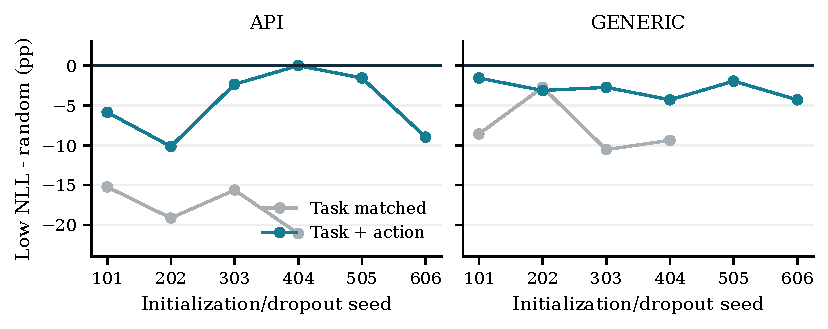
\includegraphics[width=\linewidth]{initialization-effects.pdf}
\caption{\textbf{Initialization-level effects.} Each point averages four sampling recipes. Task matching has four initialization levels; task/action matching has six. The figure shows descriptive crossed-seed outcomes and does not encode confidence intervals. Differences between curves also reflect changed content support and selection strength.}
\label{fig:initialization}
\end{figure}

\begin{table}[h]
\centering
\caption{Four prespecified task/action-study conditional repeats. Initialization 101 and recipe 101 throughout. Success rates are percentages.}
\label{tab:repeats}
\begin{tabular}{llrrr}
\toprule
Source & Policy & Original & Repeat & Change (pp)\\
\midrule
API & Random & 31.250 & 31.250 & 0.000\\
API & Low NLL & 34.375 & 29.688 & $-4.688$\\
Generic & Random & 4.688 & 6.250 & $+1.562$\\
Generic & Low NLL & 4.688 & 3.125 & $-1.562$\\
\bottomrule
\end{tabular}
\end{table}

\clearpage
\section{Scoring Geometry and Selection Sensitivity}
\label{app:scoring}
The completed diagnostic freezes 32 stress inputs: 16 selected for large recorded cache spans and 16 selected by content hash from the remainder. It evaluates canonical unpadded inputs with explicit positions and a fixed logits window, a canonical repeat, unpadded default positions, a dynamic logits window, and four padded conditions. It separately evaluates FP32 references, four direct supervised-loss checks, 392 original-layout replay observations, and uniform BF16 scores for all 853 distinct message inputs. The 1,194 forwards are fully accounted for; no retries, generated tokens, training updates, or teacher calls are included.

Canonical repeat, unpadded default-position, and dynamic-window conditions match canonical scores exactly on the 32 stress inputs. Across padded conditions, mean absolute score deviations range from 0.0362 to 0.0603 nat/token. BF16 versus FP32 deviation has mean 0.0396 and maximum 0.1630, with rank correlation 0.9857 on the selected inputs. Original batch layouts reproduce their original cached values exactly. These results quantify the instrument on the prespecified stress set; they do not estimate population error rates.

\begin{figure}[htbp]
\centering
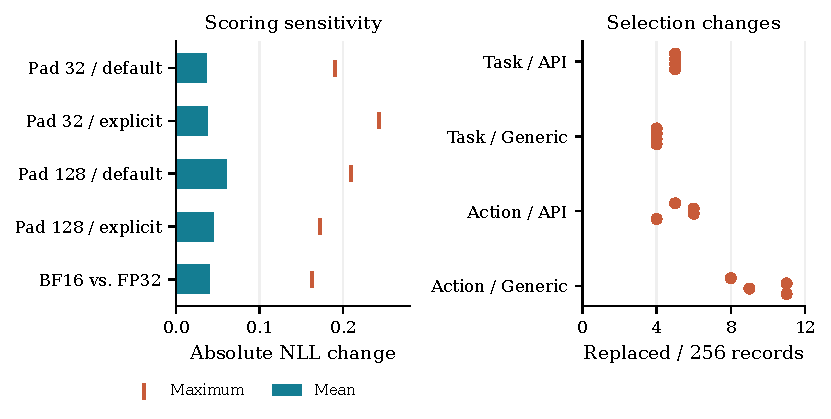
\includegraphics[width=\linewidth]{scoring-diagnostic.pdf}
\caption{\textbf{Completed scoring diagnostic.} Left: numerical layout sensitivity on the deliberately selected stress set. Right: content replacement after complete uniform rescoring, with each point a frozen selection recipe. The comparison changes the scoring procedure, not the training outcomes; the canonical-score retraining study is separate and ongoing.}
\label{fig:scoring}
\end{figure}

\begin{table}[h]
\centering
\caption{Content records replaced out of 256 after uniform rescoring. Columns are sampling-recipe seeds. Original recipes are regenerated exactly before replacement is counted.}
\label{tab:replacement}
\begin{tabular}{llrrrr}
\toprule
Control & Source & 101 & 202 & 303 & 404\\
\midrule
Task matched & API & 5 & 5 & 5 & 5\\
Task matched & Generic & 4 & 4 & 4 & 4\\
Task/action matched & API & 5 & 6 & 6 & 4\\
Task/action matched & Generic & 8 & 11 & 9 & 11\\
\bottomrule
\end{tabular}
\end{table}

\smallpara{Ongoing canonical-score replication.}
A separate freeze specifies 96 newly trained models, six initialization/dropout seeds, four recipes, two sources, and two policies, at the same 192-update budget and with the same 64 development tasks. Random indices must remain identical to the previous reference; low-NLL schedules use the completed uniform scores. Both policies are retrained, with an 18 cumulative GPU-hour cap. This study is running as of the manuscript's evidence cutoff. No interim outcome enters the completed-result comparisons in this paper.

\clearpage
\section{Second-Environment Base Calibration}
\label{app:webshop}
The WebShop pilot uses the full product/search backend and the pinned base checkpoint without an adapter. It evaluates 32 shared training goals under public ReAct and Act-only prompt ports, with at most 14 model decisions per episode and at most 100 output tokens per decision. All decisions, including thoughts and invalid controls, consume the episode budget. The backend is not queried through the ALFWorld training model servers.

\begin{table}[h]
\centering
\caption{Train-only WebShop calibration. Model-output errors are distinct from transport errors; all requests complete. This is not a post-SFT selection comparison.}
\label{tab:webshop}
\small
\begin{tabular}{lrr}
\toprule
Metric & ReAct & Act-only\\
\midrule
Goals solved / evaluated & 5/32 & 6/32\\
Success (\%) & 15.625 & 18.750\\
Mean partial score & 0.4125 & 0.4380\\
Model requests & 247 & 216\\
Physical actions & 86 & 91\\
Thought decisions & 78 & 38\\
Invalid format / invalid control & 24 / 59 & 10 / 77\\
Episodes exhausting decision budget & 10 & 10\\
Transport errors & 0 & 0\\
\bottomrule
\end{tabular}
\end{table}

\begin{figure}[htbp]
\centering
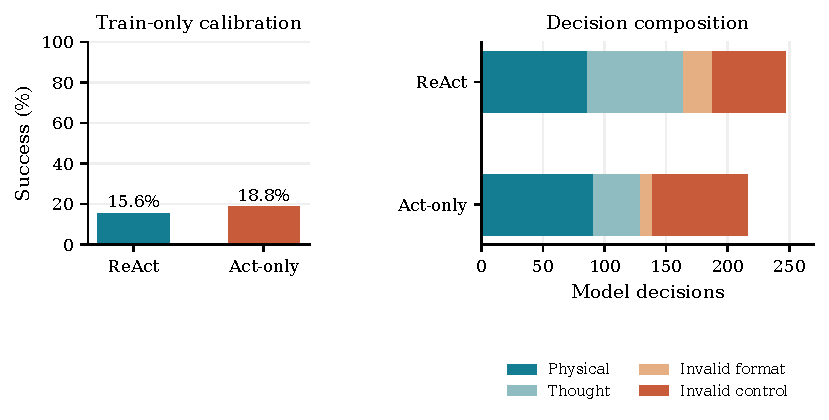
\includegraphics[width=\linewidth]{webshop-calibration.pdf}
\caption{\textbf{WebShop starting-point calibration.} Two public prompt ports on the same 32 training goals. Success-count differences of one goal do not establish prompt superiority. The composition of model decisions exposes substantial invalid-format/control behavior and informs a future learning protocol.}
\label{fig:webshop}
\end{figure}

Across both prompts the pilot records 703,520 input and 15,844 output tokens, 463 completed requests, and 243.564 GPU seconds. Teacher calls, official evaluation episodes, and optimizer updates are zero. A second-environment \emph{learning} comparison must still fix the candidate pool, selection unit, training budget, common executor, and fresh task protocol.

\clearpage
\section{Retained Baseline and Evidence Boundaries}
\label{app:baseline}
The API-versus-ReAct source study is distinct from the API/Generic pools used in the controlled selection experiments. Both source collectors make 144 attempts using the same base student. The API condition uses cached guidance from public resets; ReAct uses public examples and reasoning/action interaction. The conditions also differ in format and thought mechanism, so that comparison is a pipeline comparison, not an isolated teacher-card intervention.

Common-success matching uses 58 paired successful task/environment-seed cases and yields 452 eligible action labels per source. At 256 A-training presentations, the raw adaptation-AUC difference is $-3.564$ points. The full eligible corpora instead contain 726 API and 981 ReAct labels. A prepared 1,024-presentation schedule visits each complete corpus at least once, but its formal source-comparison study has not been executed. The old negative result remains part of the evidence and is not replaced by the within-pool selection analysis.

\smallpara{Scope relative to existing selectors.}
The implemented low-NLL policy selects action examples and uses ordinary supervised target loss. SmartAD additionally selects complete correct teacher trajectories and applies segment weighting; LESS uses target demonstrations and optimizer-aware gradient features; Rho-1 uses a reference-based token criterion. These methods require distinct implementation and cost accounting. No scores from incompatible published benchmark splits are inserted into our result table.

\smallpara{Provenance and reproducibility.}
The source bundle contains the full \LaTeX{} manuscript, editable TikZ diagrams, vector result figures, a BibTeX database, a figure/table generation script, and a hash-bound evidence manifest. Completed results are regenerated from local audited JSON reports. Raw goals, messages, scoring journals, credentials, and adapter weights are not included in the manuscript package. The official NeurIPS style is preserved byte-for-byte with its download source and SHA256. The document uses preprint mode and does not claim acceptance or submission to a particular venue.

\smallpara{Responsible reporting.}
The experiments involve simulated tasks and no new human-subject data. We use existing models, environment data, and baseline resources under their original terms. We make no real-robot, real-purchase, safety, recursive self-improvement, or state-of-the-art claim. Authors must complete venue-specific disclosures, anonymity checks, and the final checklist before an actual submission.

\end{document}
